\label{chap:requirements}
Die betrachteten Ansätze mit Verhaltensanalyse oder CV-Technik, werden für die Arbeit nicht berücksichtigt und treten nur bei der Analyse / Klassifizierung der Testdaten in Erscheinung. Gähnen, häufiges blinzeln oder abkommen von der Fahrspur, können Hinweise auf Müdigkeit sein, sodass die entsprechenden EEG-Sequenzen gelabelt werden können. 
Aufgrund seiner höheren Genauigkeit, gegenüber EKG oder EOG, wird für die Anwendung ein EEG genutzt. Ein multimodales System ist vorbereitet aber nicht umgesetzt. Die betrachteten Arbeiten zeigen in verschiedensten Ausführungen sehr gut Ergebnisse (\textasciitilde 90\% \cite{Lin05eeg-baseddrowsiness}, \cite{Subasi:2005:ARA:1707423.1707550}), sodass es sich beim EEG um eine aussichtsreiche Grundlage handelt. 
Bei der Klassifizierung lässt nutzen viele Ansätze ein Künstliches Neuronales Netz (KNN)\cite{wilson_890161}\cite{khalifa_893852}\cite{Subasi:2005:ARA:1707423.1707550} \cite{Vuckovic2002349}. Weitere Ansätze nutzen die Lineare Diskriminanten Analyse\cite{Vicente_6164509}\cite{Khushaba_5580017} oder ein SVM\cite{Park:2009:DDD:1667780.1667798}\cite{zhang_6513058}. Aufgrund der Häufigkeit in den anderen Arbeiten und der guten Bibliotheksunterstützung (PyBrain) wurde der Ansatz mit einem KNN weiter verfolgt. Alle Ansätze wurden in einer Simulierten Umgebung entwickelt und nie unter realen Bedingungen getestet. Aus der Analyse der verwandten Forschungsarbeiten ergeben sich Anforderungen an eine Anwendung zur \acl{ME}. 

Da es sich um ein sicherheitsrelevantes \acl{FAS} handelt, muss es in erster Linie präzise und korrekt funktionieren. Nicht ausgelöste Müdigkeitswarnungen wägen den Fahrer in Sicherheit, obwohl er evtl. nicht mehr in der Lage ist, sein Fahrzeug zu führen. Falsch ausgelöste Warnungen senken die Akzeptanz der Anwendung und führen im Extremfall zu deren   Abschaltung. Zudem muss es robust gegen Störungen und Falscheingaben sein, es muss zu jeder Zeit gewährleistet sein, dass das System läuft bzw. den Fahrer im Fehlerfall rechtzeitig über den Status der Anwendung informieren.

Die Anwendung muss zudem nahezu in Echtzeit funktionieren und den Fahrer sofort über eine erkannte Müdigkeit informieren. Bei der der Implementierung muss auf die Performance der Erkennung geachtet werden. Eine zu späte Meldung an den Fahrer könnte zu einem Unfall führen. Um das System möglichst flexibel zu machen, sollte es auf verschiedenen Plattformen lauffähig sein, auch hier muss eine verringerte Rechenleistung beachtet werden (bspw. auf einem Smartphone).

Um die Software möglichst flexibel bzw. unabhängig von der Hardware zu machen, sollen Datenquelle und Datenverarbeitung möglichst lose gekoppelt sein und sich leicht auf verschiedenen Systemen ausführen lassen. Das hinzufügen von weiteren Quellen (bspw. EKG oder EOG) soll vorbereitet werden.

Die Rückmeldung der Anwendung soll den Fahrer warnen, sodass er diese auf jeden Fall wahrnimmt, jedoch nicht in die Fahrsituation eingreift. Es ist mehr als Hinweis zu verstehen und nicht als Maßregelung, da dies die Akzeptanz wiederum mindern könnte. Die Anwendung soll ohne lange Einrichtung oder Interaktion des Fahrers funktionieren.

Der Komfort beim Fahren sollte möglichst hoch sein und die Sensoren sollten den Fahrer möglichst wenig beeinträchtigen. Mit einem medizinischen EEG mit 64 Pins und vielen Kabeln, ist das kaum möglich. Das Emotiv EEG lässt sich wie eine Mütze aufsetzen und überträgt seine Daten via Bluetooth - ein Komfortgewinn. Im Produktiveinsatz ist das dennoch zu unbequem und wird in dieser Form nicht in Serie gehen können.
Weiterhin soll das System unter realen Bedingungen getestet werden können und sich daher leicht vom Fahrsimulator der \acl{RTU} in ein echtes Auto oder einen anderen Simulator portieren lassen. So können Störungen während einer richtigen Autofahrt (die sich nicht simulieren lassen) erkannt werden. In einem anderen Simulator kann die Anwendung zur Validierung und Verbesserung von anderen Systeme verwendet werden.

Für ein Projekt an einer Hochschule, das auch für Folgeprojekte genutzt werden soll, ergeben sich ebenso Anforderungen an die Codequalität, insbesondere an Lesbarkeit und Wartbarkeit. Die Funktionalität und der Aufbau der Anwendung muss sauber dokumentiert werden, sodass der Einstieg für neue Entwickler möglichst reibungslos verläuft.

Wichtigste Punkte sind die Korrektheit, Portabilität und Komfort des Systems (Abb. \ref{fig:emphasis}). Wobei vor allem Portabilität und Komfort in den betrachteten Arbeiten bisher kaum berücksichtigt wurden.

\begin{figure}[h] 
  \begin{center}
    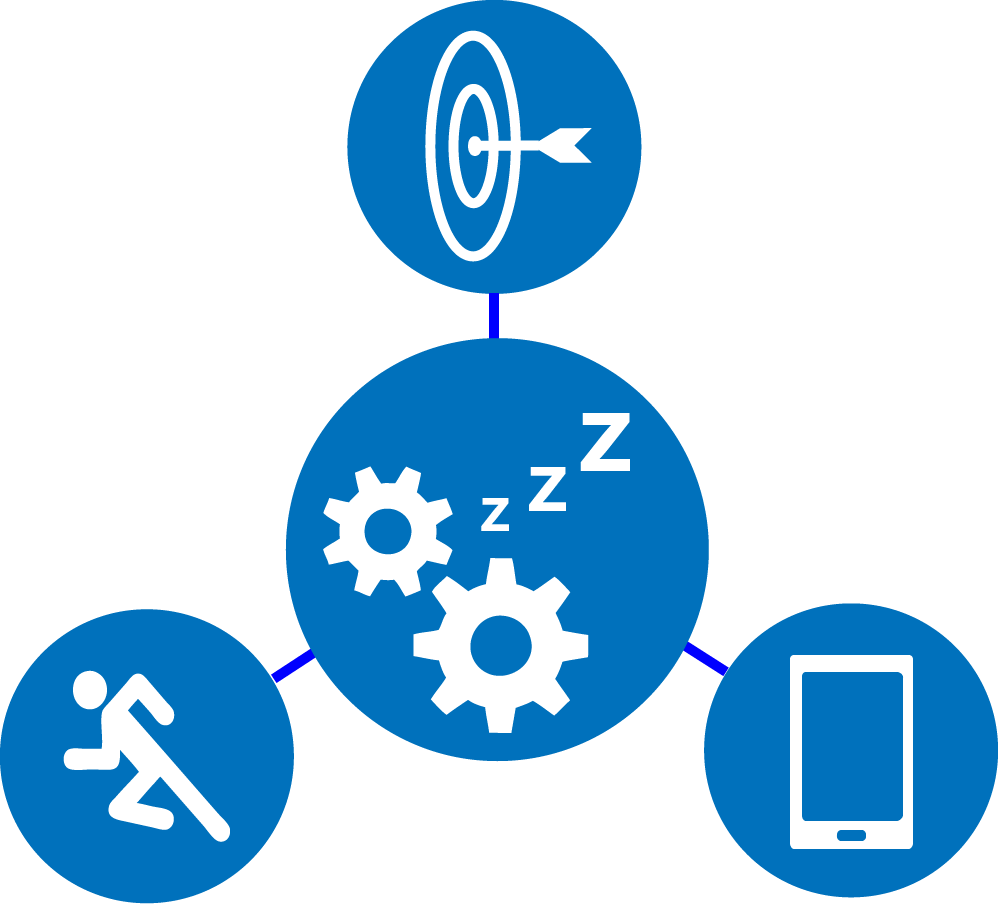
\includegraphics[width=4cm]{img/all}
    \caption[Schwerpuntke der Anwendung]{Die Anwendung mit den Schwerpunkten: Korrektheit, Portabilität und Komfort \label{fig:emphasis}}
  \end{center}
\end{figure}